\documentclass[a4paper]{article}

\usepackage[14pt]{extsizes} % чтобы использовать шрифт размером больше 12
\usepackage{cmap} % для кодировки шрифтов в pdf
\usepackage[T2A]{fontenc} % пакет указывает внутреннюю кодировку в системе LaTeX
\usepackage[utf8]{inputenc} % кодировка  
\usepackage[english, russian]{babel} % пакет для локализации

\usepackage{graphicx} % для вставки картинок
\usepackage{amssymb,amsfonts,amsmath,amsthm} % математические дополнения от АМС
\usepackage{indentfirst} % отделять первую строку раздела абзацным отступом тоже
\usepackage{makecell} % для создания таблиц
\usepackage{multirow} % для продвинутых таблиц
\usepackage{setspace} % для изменения междустрочного интервала
\usepackage{ulem} % подчеркивания
\usepackage{csvsimple} % для импорта csv - таблиц
\usepackage{siunitx,array,booktabs}
\usepackage[tableposition=top]{caption}

\usepackage[left=20mm, top=15mm, right=15mm, bottom=15mm, nohead, footskip=10mm]{geometry} % настройки полей документа

\linespread{1.3} % полуторный интервал
 
\begin{document} % начало документа
 
\section{Математическая постановка задачи}

Для решения общей задачи по нахождению деформаций и напряжений в деформируемом теле, занимающем область $G$ с границей $\partial \, G$, необходимо использовать следующие соотношения:

кинематические граничные условия
\begin{equation}
u(x) = u_0, \ x \in \partial \, G_D,
\end{equation}

силовые граничные условия
\begin{equation}
\sigma(u) \cdot n = p(x), \ x \in \partial \, G_N,
\end{equation}

соотношения Коши для тензора полных деформаций
\begin{equation}
\varepsilon(u)=\dfrac{1}{2}(\nabla u + (\nabla u)^T,
\end{equation}

тензор напряжений
\begin{equation}
\sigma(u)=???
\end{equation}

Здесь $u(x)$ - компоненты вектора перемещения, $\partial G_D$ - участок границы, на котором действуют кинематические условия Дирихле, $\partial G_N$ - участок границы, на котором действуют силовые граничные условия Неймана, $p(x)$ - вектор внешней нагрузки. 

Решить данную задачу можно с помощью метода декомпозиции Шварца.

\subsection{Методы Шварца}
Рассмотрим классическую задачу метода Шварца для двух подобластей: имеется сложная область $\Omega$, состоящая из объединения двух простых областей (круга $\Omega_1$ и прямоугольника $\Omega_2$). Рассмотрим уравнение Пуассона, цель которого найти перемещения $u: \Omega \rightarrow \mathbb{R}$ при условии, что
\begin{equation*}
\begin{array}{rl}
-\bigtriangleup \!(u) = f, & u \in \Omega \\
u = 0, & u \in \partial \Omega
\end{array}
\end{equation*}

\begin{figure}[h]
\center{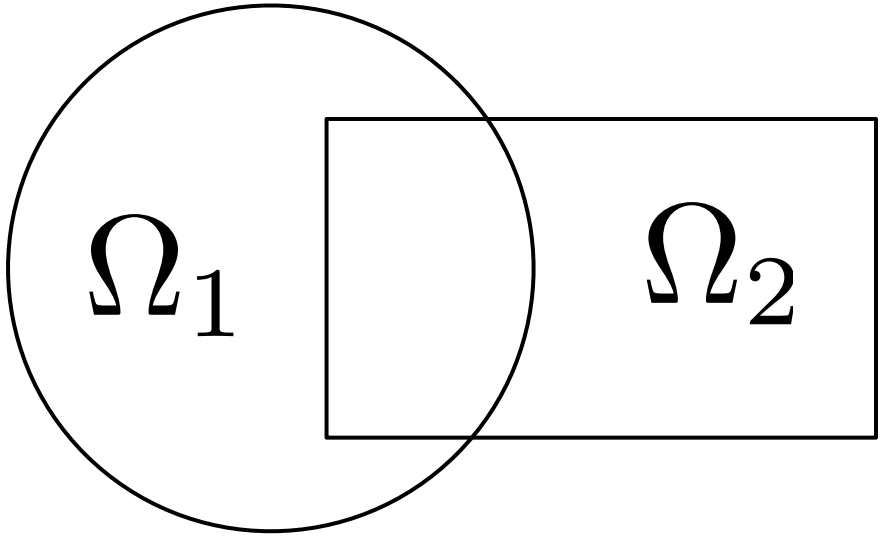
\includegraphics[scale=0.2]{img/simple_domains.png}}
\caption{Сложная область, получившаяся из объединения двух простых областей}
\label{fig:image_01}
\end{figure}

\newpage

Классический метод Шварца это итерационный метод, основанный на решении задач меньшего масштаба в подобластях $\Omega_1$ и $\Omega_2$. Один шаг итерационного процесса обновления результатов $u^n \rightarrow u^{n+1}$:
\begin{equation*}
\begin{array}{rl}
-\bigtriangleup \! (u^{n+1}) = f, & u \in \Omega_1 \\
u^{n+1} = 0, & u \in \partial \Omega_1 \cap \partial \Omega \\
u^{n+1} = u^n, & u \in \partial \Omega_1 \cap \bar{\Omega_2}
\end{array}
\textrm{после чего}
\begin{array}{rl}
-\bigtriangleup \! (u^{n+1}) = f, & u \in \Omega_2 \\
u^{n+1} = 0, & u \in \partial \Omega_2 \cap \partial \Omega \\
u^{n+1} = u^n, & u \in \partial \Omega_2 \cap \bar{\Omega_1}
\end{array}
\end{equation*}

Теперь же рассмотрим случай для произвольной области и произвольного числа подобластей. Вернёмся к нашей первоначальной задаче (ссылка здесь), представим область $G$ в виде объединения конечного числа подобластей $G = \bigcup_{i=1}^{M} G_i$ с конечным числом границ $\partial G_1, \ldots, \partial G_M$, где M - число подобластей. Данные подобласти пересекаются, что требует ввода дополнительных обозначений для границ, возникающих после декомпозиции областей: $\Gamma = \bigcup_{i=1}^{M} \Gamma_i$. 

Выберем начальное приближение для перемещений, удовлетворяющее граничным условиям (ссылка здесь). Алгоритм из классического метода Шварца можно оптимизировать для большего числа подобластей:
\begin{equation*}
\begin{array}{rl}
-\bigtriangleup \! (u^{n+\frac{i}{M}}) = f(x), & x \in G_i \\
\sigma(u^{n+\frac{i}{M}}) \cdot n = p(x), & x \in \partial G_N \cap \partial G_i \\
u^{n+\frac{i}{M}}(x) = 0, & x \in \partial G_D \cap \partial G_i \\ 
u^{n+\frac{i}{M}}(x) = u^{n+\frac{(i - 1)}{M}}(x), & x \in G \setminus ((G_i \setminus \partial G_i) \cap (\partial G_N \cup \partial G_i))
\end{array}
\end{equation*}

Данный алгоритм Шварца называют мультипликативным, он последовательный и решение на каждой подобласти зависит от решения на предыдущей подобласти (или от решения на предыдущей итерации, если речь идёт о первой подобласти для итерации).

Существует также другой вариант метода Шварца, основанный на решении локальных задач для каждой подобласти без зависимости от соседних подобластей:
\begin{equation*}
\begin{array}{rl}
-\bigtriangleup \! (u^{n+\frac{i}{M}}) = f(x), & x \in G_i \\
\sigma(u^{n+\frac{i}{M}}) \cdot n = p(x), & x \in \partial G_N \cap \partial G_i \\
u^{n+\frac{i}{M}}(x) = 0, & x \in \partial G_D \cap \partial G_i \\ 
u^{n+1}(x) = u^{n}(x), & x \in G \setminus ((G_i \setminus \partial G_i) \cap (\partial G_N \cup \partial G_i))
\end{array}
\end{equation*}

Этот метод называется аддитивный метод Шварца. В конце каждой итерации решение вычисляется по формуле 
\begin{equation*}
u^{n+1} = u^{n} + \alpha \sum_{i=1}^{M} (u_i^{n+1} - u^{n}),
\end{equation*}
где коэффициент $\alpha$ - некоторый параметр, от которого зависит скорость сходимости итерационного процесса. 

\newpage

\section{Результаты численных расчётов}

В данном разделе будут приведены расчёты четырёх тестовых задач с использованием четырёх методов. Для каждой из задач для базового случая будут приведены графики распределения напряжений вдоль поверхности, к которой приложено давление, а также графики распределения перемещений на всей расчётной области.

Для методов декомпозиции области расчётные области будут разбиты на заданное количество секторов без перекрытия $\Omega_1, \ldots, \Omega_M$ в зависимости от задачи, где M - число подобластей. Также стоит заметить, что каждая подобласть $\Omega_i$ ($i = 1,\ldots,M$) в зависимости от задачи обладает своими размерными характеристиками. Подобласть $G_i$ соответствует объединению подобласти $\Omega_i$ и дополнительных участков соседних подобластей $\Omega_{i-1}$ и $\Omega_{i+1}$. Размеры этих дополнительных участков зависят от относительного коэффициента перекрытия (отношение размера перекрытия к размеру подобласти $\Omega_i$).

Итерационный процесс для мультипликативного, аддитивного и двухуровневого аддитивного методов продолжался до тех пор, пока не выполнялось условие критерия останова:

\begin{equation}
u_error = \sqrt{\frac{\sum_{k = 1}^{N_{p}} s_k \left(\frac{u_{k}^{m+1} - u_{k}^{m}}{u_{k}^{m+1}} \right)^2}{\sum_{k = 1}^{N_{p}} s_k}} < \varepsilon_0,
\end{equation}
где $s_k$ - суммарная площадь элементов сетки, в которые входит $k$-й узел, разделённая на количество узлов в элементе, $N_{elem}$ - количество узлов сетки, $u_{k}^{m+1}$ - решение на текущей итерации, $u_{k}^{m}$ - решение на предыдущей итерации.

Дополнительно для каждой из задач для методов декомпозиции будут приведены таблицы зависимости количества итераций от относительного коэффициента перекрытия.

\subsection{Первая тестовая задача}

Расчётная область - тело, закреплённое с левой и правой стороны по оси OX и с нижней стороны по оси OY. Сверху действует распределённая нагрузка $p = 50$ МПа. Ширина тела $a = 2$ см, высота тела $b = 1$ см. 

\begin{figure}[h]
\center{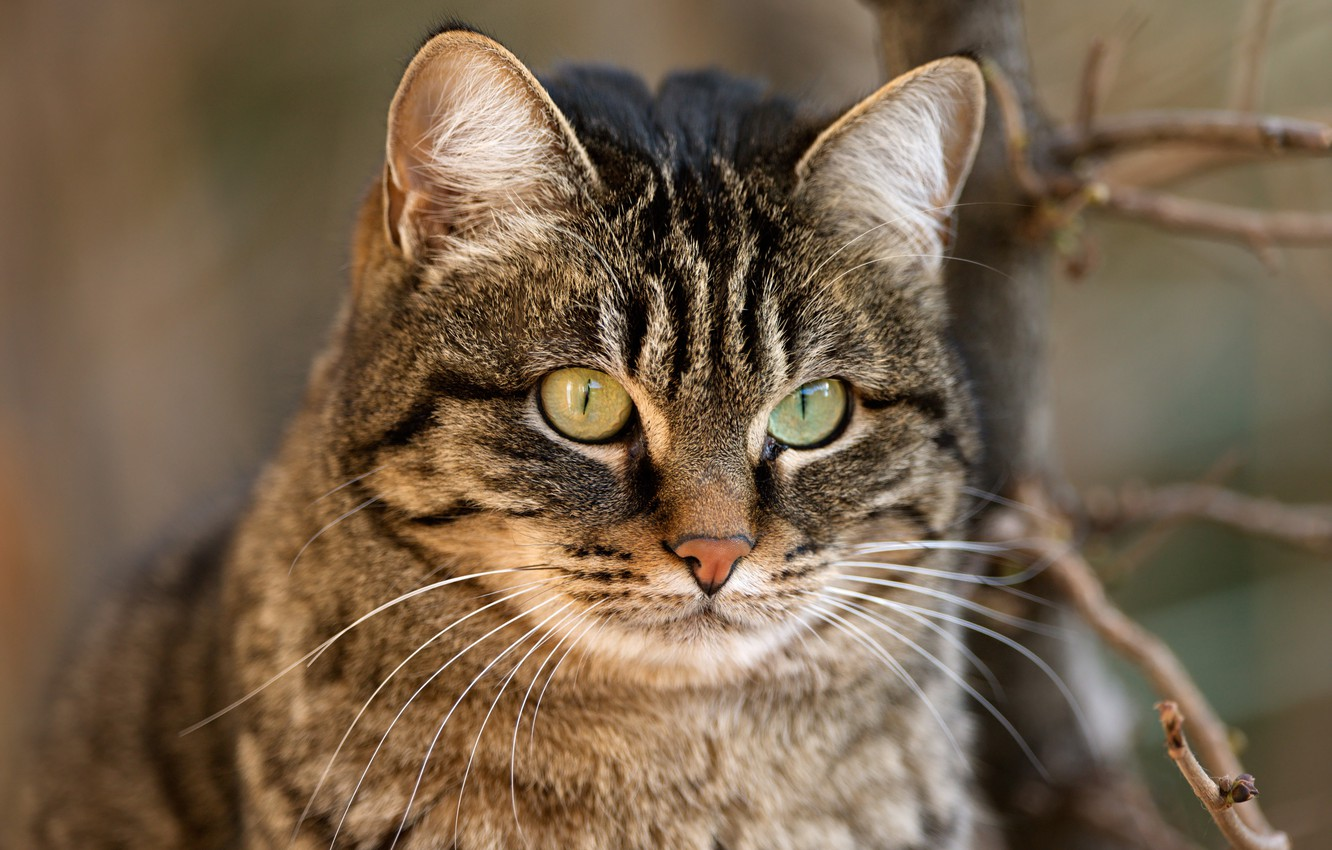
\includegraphics[scale=0.2]{img/task_01_scheme.jpg}}
\caption{Схема расчётной области первой тестовой задачи (заглушка)}
\label{fig:task_01_scheme}
\end{figure}

Для решения поставленной задачи примем, что материал тела имеет следующие параметры: модуль Юнга $E = 70$ ГПа, коэффициент Пуассона $\mu = 0.34$. 

Для исследования зависимости сходимости метода от размерности итоговой системы линейных уравнений рассмотрены три расчётные сетки с шагами $h = 0.05$ (количество узлов - 994), $h = 0.025$ (количество узлов - 3812), $h = 0.0125$ (количество узлов - 15006). Для аддитивного метода Шварца итерационный параметр $\alpha = 0.5$.

Для данной задачи известны аналитические решения для компонент тензора напряжений и для перемещений. В таблице 1 представлены нормы ошибок вычислений перемещений, радиального и окружного напряжений, полученные при решении задачи без декомпозиции для различных сеток, в таблице 2 - отношения норм ошибок.

\newpage

\subsection{Третья тестовая задача}

Расчётная область - сектор поперечного сечения толстостенной трубы, основные размерные характеристики трубы - внутренний радиус $r_1 = 1$ см, внешний радиус $r_2 = 2$ см. К внутреннему торцу приложено давление $p_1 = 5$ МПа, к внешнему торцу также приложено давление $p_2 = 10$ МПа.

\begin{figure}[h]
\center{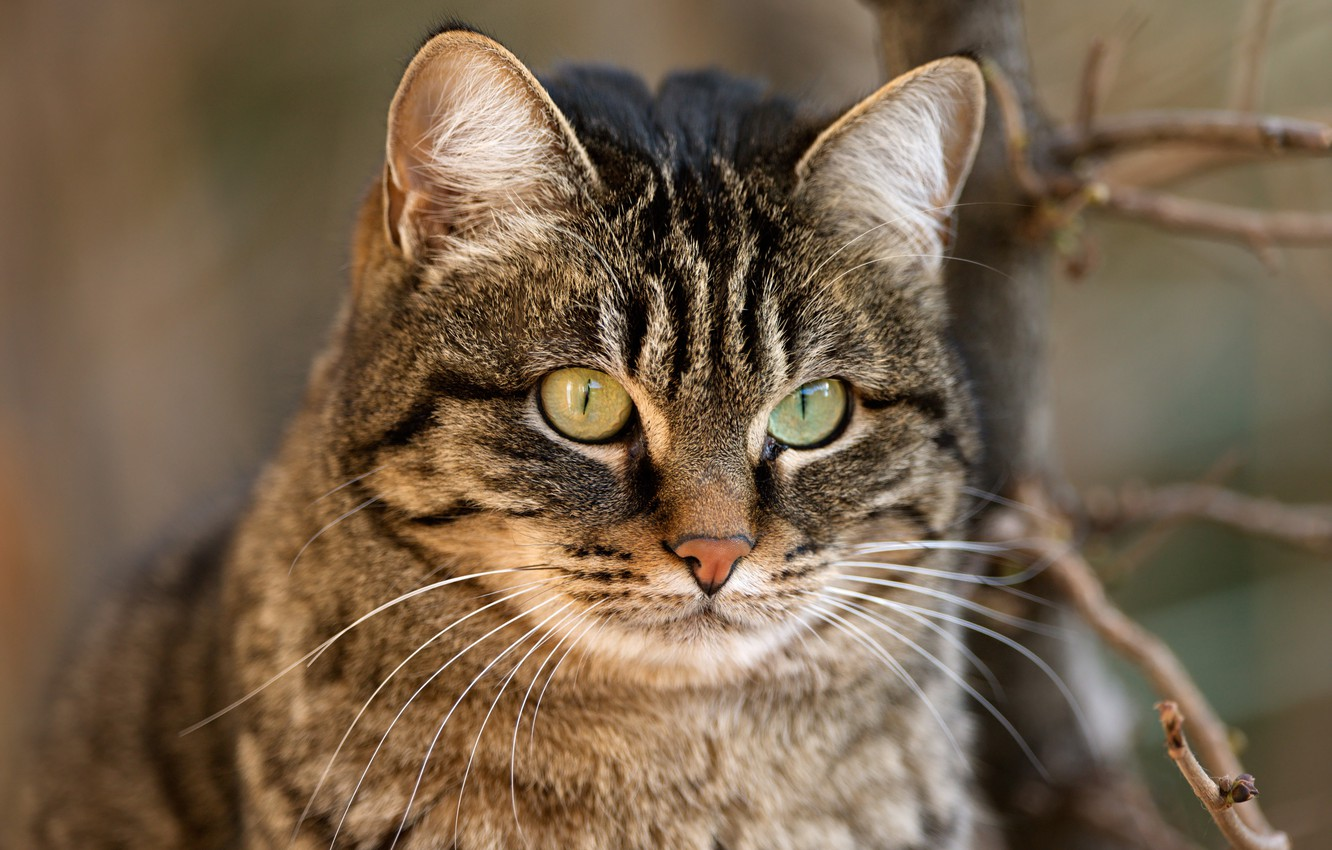
\includegraphics[scale=0.2]{img/task_04_scheme.jpg}}
\caption{Схема расчётной области четвёртой тестовой задачи (заглушка)}
\label{fig:task_04_scheme}
\end{figure}

Для применения методов декомпозиции области исходная область разбивалась на заданное количество секторов без перекрытия $\Omega_1, \ldots, \Omega_M$, где M - число подобластей. Размеры участков, а именно центральный угол каждого из них, задавался заранее выбранным коэффициентом относительного перекрытия.

Для решения поставленной задачи примем, что материал тела имеет следующие параметры: модуль Юнга $E = 70$ ГПа, коэффициент Пуассона $\mu = 0.34$. Для данной задачи известны аналитические решения для компонент тензора напряжений и для перемещений.

Для аддитивного метода Шварца итерационный параметр $\alpha = 0.5$. Для исследования зависимости сходимости метода от размерности итоговой системы линейных уравнений рассмотрены три расчётные сетки с шагами $h = 0.05$ (количество узлов - 1334), $h = 0.025$ (количество узлов - 4571), $h = 0.0125$ (количество узлов - 16636).

\subsubsection{Мультипликативный метод Шварца}

В таблице (\ref{table:task_3_mult_iters}) представлено количество итераций в зависимости от количества подобластей и шага сетки при использовании мультипликативного метода Шварца в случае фиксированного относительного перекрытия подобластей (данный коэффициент равен 0.3). Анализ полученных результатов показал, что:
\begin{itemize}
\item при увеличении числа подобластей количество итераций увеличивается;
\end{itemize}

\begin{table}[h]
\caption{Количество итераций в зависимости от количества подобластей}
\csvloop{
	file = ../results/thick_walled_cylinder/pressure_only/iterations/schwarz_multiplicative.csv,
	head to column names,
	before reading = \centering\sisetup{table-number-alignment=center},
	tabular = {
		@{} |
		c |
		c | 
		c |
		c |
		@{}
	},
	table head = \hline Количество подобластей & \text{h = 0.5} & \text{h = 0.025} & \text{h = 0.0125} \\\hline,
	command = \amnt & \first & \second & \third,
	late after line = \\\hline
}
\label{table:task_3_mult_iters}
\end{table}

\subsubsection{Аддитивный метод Шварца}

В таблице (\ref{table:task_3_add_iters}) представлено количество итераций в зависимости от количества подобластей и шага сетки при использовании аддитивного метода Шварца в случае фиксированного относительного перекрытия подобластей (данный коэффициент равен 0.3). Анализ полученных результатов показал, что:
\begin{itemize}
\item при увеличении числа подобластей количество итераций существенно возрастает;
\end{itemize}

\begin{table}[h]
\caption{Количество итераций в зависимости от количества подобластей}
\csvloop{
	file = ../results/thick_walled_cylinder/pressure_only/iterations/schwarz_additive.csv,
	head to column names,
	before reading = \centering\sisetup{table-number-alignment=center},
	tabular = {
		@{} |
		c |
		c | 
		c |
		c |
		@{}
	},
	table head = \hline Количество подобластей & \text{h = 0.5} & \text{h = 0.025} & \text{h = 0.0125} \\\hline,
	command = \amnt & \first & \second & \third,
	late after line = \\\hline
}
\label{table:task_3_add_iters}
\end{table}

\subsubsection{Двухуровневый аддитивный метод Шварца}

В таблице (\ref{table:task_3_2add_iters}) представлено количество итераций в зависимости от количества подобластей и шага сетки при использовании двухуровневого аддитивного метода Шварца в случае фиксированного относительного перекрытия подобластей (данный коэффициент равен 0.3). Анализ полученных результатов показал, что:
\begin{itemize}
\item количество итераций несильно зависит от шага сетки;
\item при увеличении числа подобластей количество итераций меняется, но не так сильно по сравнению с применением аддитивного метода Шварца;
\end{itemize}

\begin{table}[h]
\caption{Количество итераций в зависимости от количества подобластей}
\csvloop{
	file = ../results/thick_walled_cylinder/pressure_only/iterations/schwarz_additive_two_level.csv,
	head to column names,
	before reading = \centering\sisetup{table-number-alignment=center},
	tabular = {
		@{} |
		c |
		c | 
		c |
		c |
		@{}
	},
	table head = \hline Количество подобластей & \text{h = 0.5} & \text{h = 0.025} & \text{h = 0.0125} \\\hline,
	command = \amnt & \first & \second & \third,
	late after line = \\\hline
}
\label{table:task_3_2add_iters}
\end{table}

\newpage

\subsection{Четвёртая тестовая задача}

Расчётная область - сектор поперечного сечения подшипника, основные размерные характеристики подшипника - центральный угол - $90^{\circ}$, внутренний радиус внутреннего кольца $r_{in}^a$ = 1.0 см, внешний радиус внешнего кольца $r_{out}^b$ = 2.0 см. Прочие характеристики, а именно внешний радиус внутреннего кольца $r_{out}^a$, внутренний радиус внешнего кольца $r_{in}^b$ и радиус шарика в полости, зависят от количества шариков в полости между кольцами.

(Тут нужно расписать, как выбирается параметр для оставшихся характеристик)

\begin{figure}[h]
\center{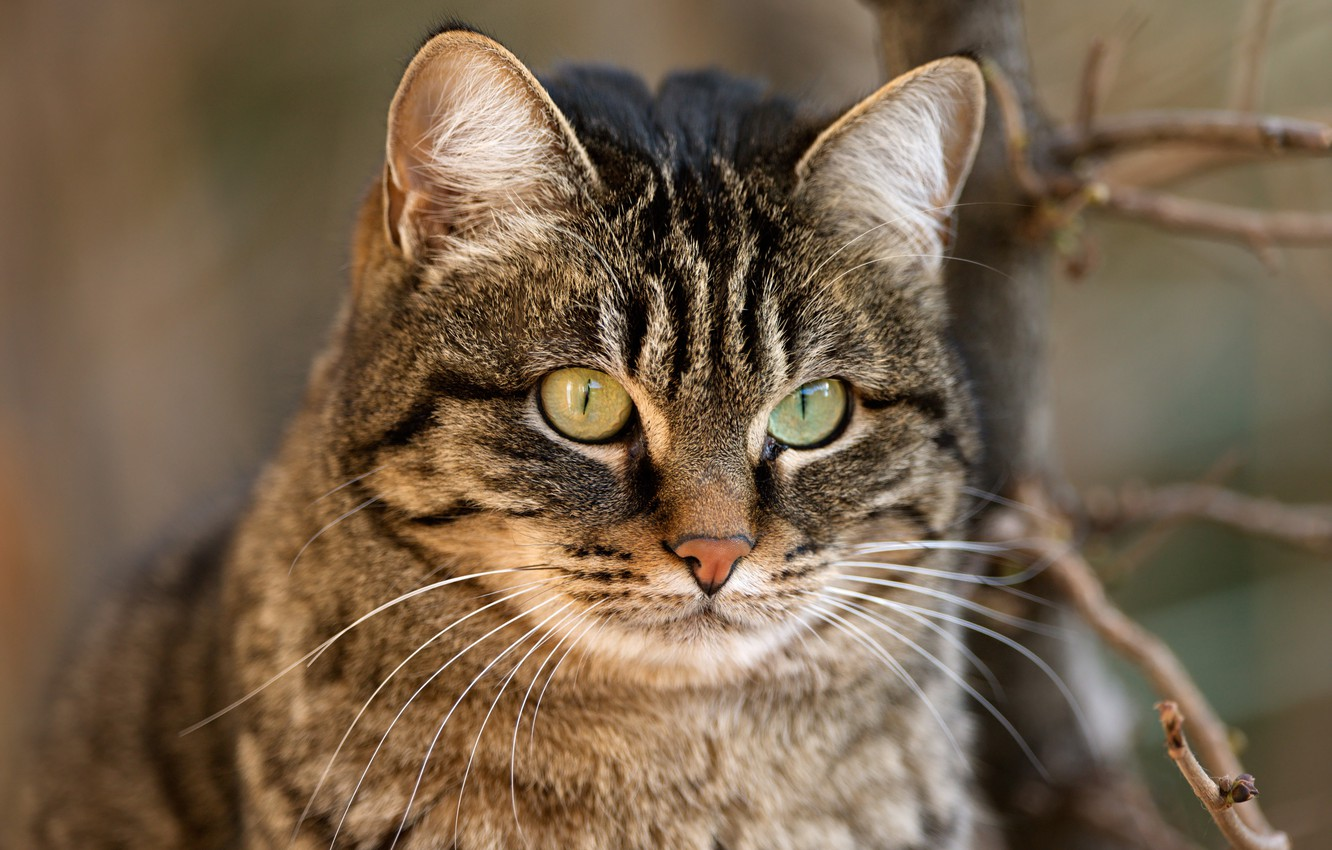
\includegraphics[scale=0.2]{img/task_04_scheme.jpg}}
\caption{Схема расчётной области четвёртой тестовой задачи (заглушка)}
\label{fig:task_04_scheme}
\end{figure}

Для применения методов декомпозиции области исходная область разбивалась на заданное количество секторов без перекрытия $\Omega_1, \ldots, \Omega_M$, где M - число подобластей. Размеры участков, а именно центральный угол каждого из них, задавался заранее выбранным коэффициентом относительного перекрытия.

Для решения поставленной задачи примем, что материал тела имеет следующие параметры: модуль Юнга $E = 210$ ГПа, коэффициент Пуассона $\mu = 0.25$. Для данной задачи неизвестны аналитические решения для компонент тензора напряжений и для перемещений.

Для аддитивного метода Шварца итерационный параметр $\alpha = 0.5$. Для исследования зависимости сходимости метода от размерности итоговой системы линейных уравнений рассмотрены три расчётные сетки с шагами $h = 0.05$ (количество узлов - 1334), $h = 0.025$ (количество узлов - 4571), $h = 0.0125$ (количество узлов - 16636).


\subsubsection{Мультипликативный метод Шварца}

В таблице (\ref{table:task_4_mult_iters}) представлено количество итераций в зависимости от количества подобластей и шага сетки при использовании мультипликативного метода Шварца в случае фиксированного относительного перекрытия подобластей (данный коэффициент равен 0.3). Анализ полученных результатов показал, что:
\begin{itemize}
\item при увеличении числа подобластей количество итераций увеличивается;
\end{itemize}

\begin{table}[h]
\caption{Количество итераций в зависимости от количества подобластей}
\csvloop{
	file = ../results/bearing/pressure_only/iterations/schwarz_multiplicative.csv,
	head to column names,
	before reading = \centering\sisetup{table-number-alignment=center},
	tabular = {
		@{} |
		c |
		c | 
		c |
		c |
		@{}
	},
	table head = \hline Количество подобластей & \text{h = 0.5} & \text{h = 0.025} & \text{h = 0.0125} \\\hline,
	command = \amnt & \first & \second & \third,
	late after line = \\\hline
}
\label{table:task_4_mult_iters}
\end{table}

\subsubsection{Аддитивный метод Шварца}

В таблице (\ref{table:task_4_add_iters}) представлено количество итераций в зависимости от количества подобластей и шага сетки при использовании аддитивного метода Шварца в случае фиксированного относительного перекрытия подобластей (данный коэффициент равен 0.3). Анализ полученных результатов показал, что:
\begin{itemize}
\item при увеличении числа подобластей количество итераций существенно возрастает;
\end{itemize}

\begin{table}[h]
\caption{Количество итераций в зависимости от количества подобластей}
\csvloop{
	file = ../results/thick_walled_cylinder/pressure_only/iterations/schwarz_additive.csv,
	head to column names,
	before reading = \centering\sisetup{table-number-alignment=center},
	tabular = {
		@{} |
		c |
		c | 
		c |
		c |
		@{}
	},
	table head = \hline Количество подобластей & \text{h = 0.5} & \text{h = 0.025} & \text{h = 0.0125} \\\hline,
	command = \amnt & \first & \second & \third,
	late after line = \\\hline
}
\label{table:task_4_add_iters}
\end{table}

\subsubsection{Двухуровневый аддитивный метод Шварца}

В таблице (\ref{table:task_4_2add_iters}) представлено количество итераций в зависимости от количества подобластей и шага сетки при использовании двухуровневого аддитивного метода Шварца в случае фиксированного относительного перекрытия подобластей (данный коэффициент равен 0.3). Анализ полученных результатов показал, что:
\begin{itemize}
\item количество итераций несильно зависит от шага сетки;
\item при увеличении числа подобластей количество итераций меняется, но не так сильно по сравнению с применением аддитивного метода Шварца;
\end{itemize}

\begin{table}[h]
\caption{Количество итераций в зависимости от количества подобластей}
\csvloop{
	file = ../results/bearing/pressure_only/iterations/schwarz_additive_two_level.csv,
	head to column names,
	before reading = \centering\sisetup{table-number-alignment=center},
	tabular = {
		@{} |
		c |
		c | 
		c |
		c |
		@{}
	},
	table head = \hline Количество подобластей & \text{h = 0.5} & \text{h = 0.025} & \text{h = 0.0125} \\\hline,
	command = \amnt & \first & \second & \third,
	late after line = \\\hline
}
\label{table:task_4_2add_iters}
\end{table}

% \csvloop{
%	file = ../results/bearing/pressure_only/iterations/schwarz_additive.csv,
%	head to column names,
%	before reading = \centering\sisetup{table-number-alignment=center},
%	tabular = {
%		@{} |
%		c |
%		c | 
%		c |
%		c |
%		@{}
%	},
%	table head = \hline Количество подобластей & \text{h = 0.5} & \text{h = 0.025} & \text{h = 0.0125} \\\hline,
%	command = \amnt & \first & \second & \third,
%	late after line = \\\hline
% }




\end{document}
